\section{伴随算子}
\label{sec:lop-adjoint}

矩阵有共轭转置，它在算子上的对应物叫做伴随。定义的动机来自观测：算子$T:H_1\to H_2$把输入送进输出空间，我们却常常只能用一个测试方向去观察输出，例如读出$Tx$在某个单位向量$v$上的分量$\langle v,Tx\rangle$。

这个读数对$x$是线性的，因而是输入空间上的一个泛函。第~\ref{chap:linear-functionals}章说明，Hilbert空间上的连续线性泛函都可以写成内积；于是每个输出方向$v$都对应输入空间中的一个方向。本节用这一对应定义伴随，并研究输入中哪些方向在输出中看不见、输出中哪些方向够不着。

本节设$H_1,H_2,H_3$是同一标量域上的Hilbert空间，算子都定义在整个输入空间上并且有界。复内积沿用第~\ref{chap:function-inner-product-spaces}章的约定：对第一个变量共轭线性，对第二个变量线性。

\subsection{伴随的定义}
\label{sec:lop-adjoint-def}

固定$T\in\mathcal B(H_1,H_2)$与输出方向$v\in H_2$，考察读数$x\mapsto\langle v,Tx\rangle$。它对$x$线性，并且
\[
 \lvert\langle v,Tx\rangle\rvert\leq\lVert v\rVert\,\lVert T\rVert\,\lVert x\rVert,
\]
所以是$H_1$上的有界线性泛函。由Riesz表示定理，存在唯一的$w\in H_1$，使$\langle v,Tx\rangle=\langle w,x\rangle$对一切$x\in H_1$成立。这个$w$随$v$而定。

\begin{definition}[伴随算子]
\label{def:lop-adjoint}
设$T\in\mathcal B(H_1,H_2)$。对每个$v\in H_2$，令$T^*v\in H_1$为满足
\begin{equation}
 \langle v,Tx\rangle_{H_2}=\langle T^*v,x\rangle_{H_1}\qquad(x\in H_1)
 \label{eq:lop-adjoint}
\end{equation}
的唯一元素。映射$T^*:H_2\to H_1$称为$T$的\term{伴随}（adjoint）算子。
\end{definition}

伴随把测试方向从输出空间拉回输入空间：用$v$测试$Tx$，相当于用$T^*v$测试$x$。它的定义域是整个输出空间$H_2$，取值空间是输入空间$H_1$，方向与$T$相反；它不是从输出恢复输入，后面的移位算子会说明这一区别。

\begin{theorem}[伴随的基本性质]
\label{thm:lop-adjoint-properties}
设$S,T\in\mathcal B(H_1,H_2)$，$R\in\mathcal B(H_2,H_3)$，$\alpha\in\mathbb F$。则$T^*\in\mathcal B(H_2,H_1)$，并且
\begin{equation}
 \begin{gathered}
 (S+T)^*=S^*+T^*,\quad(\alpha T)^*=\bar\alpha T^*,\quad(RT)^*=T^*R^*,\\
 T^{**}=T,\quad\lVert T^*\rVert=\lVert T\rVert,\quad\lVert T^*T\rVert=\lVert T\rVert^2 .
 \end{gathered}
 \label{eq:lop-adjoint-properties}
\end{equation}
\end{theorem}

\begin{proof}
先证线性。对$v_1,v_2\in H_2$及标量$\beta_1,\beta_2$，由内积对第一个变量共轭线性，
\[
 \begin{aligned}
 \langle T^*(\beta_1v_1+\beta_2v_2),x\rangle
 &=\langle\beta_1v_1+\beta_2v_2,Tx\rangle\\
 &=\bar\beta_1\langle T^*v_1,x\rangle+\bar\beta_2\langle T^*v_2,x\rangle\\
 &=\langle\beta_1T^*v_1+\beta_2T^*v_2,x\rangle ,
 \end{aligned}
\]
对一切$x$成立，由表示的唯一性得线性。

和、数乘与复合的公式用同样的方式验证。复合的情形是
\[
 \langle v,RTx\rangle=\langle R^*v,Tx\rangle=\langle T^*R^*v,x\rangle.
\]
数乘公式中出现$\bar\alpha$，是因为把标量移进第一个变量要取共轭：
\[
 \langle v,\alpha Tx\rangle=\alpha\langle T^*v,x\rangle=\langle\bar\alpha T^*v,x\rangle.
\]

再证有界与范数。由式~\eqref{eq:lop-adjoint}，
\[
 \lVert T^*v\rVert^2=\langle T^*v,T^*v\rangle=\langle v,TT^*v\rangle\leq\lVert v\rVert\,\lVert T\rVert\,\lVert T^*v\rVert,
\]
两边约去$\lVert T^*v\rVert$（它为零时不等式自然成立），即得$\lVert T^*\rVert\leq\lVert T\rVert$。

对式~\eqref{eq:lop-adjoint}两边取共轭得$\langle x,T^*v\rangle=\langle Tx,v\rangle$，这说明$T$满足$T^*$的伴随所需的等式，故$T^{**}=T$。把刚才的不等式用于$T^*$，就得到反方向的$\lVert T\rVert\leq\lVert T^*\rVert$。

最后，由复合的范数估计，
\[
 \lVert T^*T\rVert\leq\lVert T^*\rVert\,\lVert T\rVert=\lVert T\rVert^2.
\]
另一方面对单位向量$x$，
\[
 \lVert Tx\rVert^2=\langle x,T^*Tx\rangle\leq\lVert T^*T\rVert,
\]
取上确界得$\lVert T\rVert^2\leq\lVert T^*T\rVert$。
\end{proof}

在$\mathbb C^n$与$\mathbb C^m$上配标准内积$\langle\bm v,\bm w\rangle=\bm v^*\bm w$，矩阵$\bm A$满足
\[
 \langle\bm v,\bm A\bm x\rangle=\bm v^*\bm A\bm x=(\bm A^*\bm v)^*\bm x,
\]
所以它的伴随是共轭转置$\bm A^*$；实情形就是转置。共轭来自内积约定本身，不能把伴随只当作“转置”的记号：在复空间中直接用转置，等式~\eqref{eq:lop-adjoint}一般不成立。式~\eqref{eq:lop-matrix-entry}的矩阵元素同样满足$(T^*)_{mn}=\overline{A_{nm}}$。

\paragraph{累积积分的伴随}
在$L^2(0,1)$上令$(Vf)(s)=\int_0^sf(t)\,\mathrm dt$，即从$0$累积到$s$。它是核为$\mathbf 1_{\{t<s\}}$的积分算子，核在$[0,1]^2$上平方可积，由定理~\ref{thm:lop-hs-bounded}有界。按矩阵看，第$s$行在列$t<s$处都是$1$，这是一个下三角矩阵。

转置以后应当是上三角矩阵。对$g\in L^2(0,1)$，被积函数$\overline{g(s)}f(t)\mathbf 1_{\{t<s\}}$在单位正方形上可积，由Fubini定理交换积分次序，
\[
 \begin{aligned}
 \langle g,Vf\rangle
 &=\int_0^1\overline{g(s)}\int_0^sf(t)\,\mathrm dt\,\mathrm ds\\
 &=\int_0^1\overline{\Bigl(\int_t^1g(s)\,\mathrm ds\Bigr)}f(t)\,\mathrm dt ,
 \end{aligned}
\]
所以$(V^*g)(t)=\int_t^1g(s)\,\mathrm ds$，即从$t$累积到$1$。

用$f=g=1$核对。左边是
\[
 \langle1,V1\rangle=\int_0^1s\,\mathrm ds=\frac12.
\]
又$V^*1=1-t$，右边是
\[
 \langle V^*1,1\rangle=\int_0^1(1-t)\,\mathrm dt=\frac12,
\]
两边相等。

\paragraph{伴随不是逆}
在$\ell^2$上，右移$S$的伴随是左移
\[
 S^*(y_1,y_2,\ldots)=(y_2,y_3,\ldots),
\]
逐项核对即得
\[
 \langle y,Sx\rangle=\sum_{k\geq1}\bar y_{k+1}x_k=\langle S^*y,x\rangle.
\]
矩阵上，$S$的$1$在主对角线下方一条斜线，转置后移到上方一条斜线。

于是$S^*S=I$，左移撤销了右移。但$SS^*(y_1,y_2,\ldots)=(0,y_2,y_3,\ldots)$抹掉了第一个坐标，$SS^*\neq I$。$S$保持长度，不丢失信息，只是它的像缺少$e_1$方向，所以$S^*$只是左逆。

这个例子同时说明无限维中单射不等于满射：$S$是单射而非满射，$S^*$是满射而非单射。对一般算子，伴随连左逆都不是：零算子的伴随仍是零算子。

\subsection{像与零空间的正交关系}
\label{sec:lop-range-kernel}

伴随的定义式把“输出方向$v$与一切$Tx$正交”翻译成输入空间中的条件$\langle T^*v,x\rangle=0$对一切$x$成立，也就是$T^*v=0$。由此得到像与零空间之间的正交关系。

\begin{theorem}[像与零空间的正交关系]
\label{thm:lop-range-kernel}
设$T\in\mathcal B(H_1,H_2)$。则
\begin{equation}
 (\operatorname{Ran}T)^\perp=\ker T^*,\qquad\overline{\operatorname{Ran}T}=(\ker T^*)^\perp ,
 \label{eq:lop-range-kernel}
\end{equation}
交换$T$与$T^*$的角色，又有$(\operatorname{Ran}T^*)^\perp=\ker T$与$\overline{\operatorname{Ran}T^*}=(\ker T)^\perp$。
\end{theorem}

\begin{proof}
$v\in(\operatorname{Ran}T)^\perp$当且仅当对一切$x$有$\langle v,Tx\rangle=0$，即$\langle T^*v,x\rangle=0$对一切$x$成立。取$x=T^*v$可知这等价于$T^*v=0$。这证明了第一个等式。

对第二个等式，只需说明线性子空间$M$满足$(M^\perp)^\perp=\overline M$，再取$M=\operatorname{Ran}T$。由定义$M\subseteq(M^\perp)^\perp$，后者是闭集，所以$\overline M\subseteq(M^\perp)^\perp$。

反过来，设$v\in(M^\perp)^\perp$，作正交分解$v=P_{\overline M}v+z$，其中$z\perp\overline M$，从而$z\in M^\perp$。$v$与$P_{\overline M}v$都与$z$正交，所以
\[
 \lVert z\rVert^2=\langle z,v-P_{\overline M}v\rangle=0,
\]
即$v\in\overline M$。其余两式把$T$换成$T^*$并用$T^{**}=T$即得。
\end{proof}

由此得到两个空间的正交分解
\begin{equation}
 H_1=\ker T\oplus\overline{\operatorname{Ran}T^*},\qquad H_2=\ker T^*\oplus\overline{\operatorname{Ran}T}.
 \label{eq:lop-four-subspaces}
\end{equation}
$\ker T$中的输入方向在输出中完全看不见，加到任何输入上都不改变输出。$\overline{\operatorname{Ran}T}$是能被输出逼近的方向。$\ker T^*$中的输出方向与一切输出正交，任何输入都到达不了。

图~\ref{fig:lop-four-subspaces}把四个子空间放在一起。这是矩阵的“四个基本子空间”在Hilbert空间中的形式，区别在于像必须取闭包。

\begin{BookInlineFigure}
  \centering
  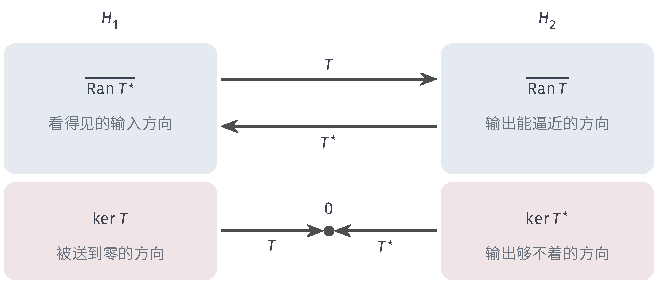
\includegraphics[width=111.404mm]{figures/04-spaces-measures-and-geometry/03-function-spaces/tikz/lop-four-subspaces/figure.pdf}
  \caption{伴随与像、零空间的正交关系。输入空间$H_1$分解为$\overline{\operatorname{Ran}T^*}$与$\ker T$，输出空间$H_2$分解为$\overline{\operatorname{Ran}T}$与$\ker T^*$。$T$把$\ker T$送到零，其余方向的像落在$\operatorname{Ran}T$中；$T^*$把$\ker T^*$送到零。无限维中像未必闭，正交关系只确定像的闭包。}
  \label{fig:lop-four-subspaces}
\end{BookInlineFigure}

\paragraph{像稠密而不闭}
闭包在无限维中不能省去。回到$\ell^2$上的对角算子$A(x_n)=(x_n/n)$。逐项核对可知$A^*=A$，且$A$是单射，所以$\ker A^*=\{0\}$，由式~\eqref{eq:lop-range-kernel}，$\operatorname{Ran}A$在$\ell^2$中稠密。

考察$y=(1/n)$，它满足$\sum_n1/n^2<\infty$，属于$\ell^2$。若$Ax=y$，逐个坐标比较得$x_n=1$，这个唯一的候选不是平方可和的，所以$y\notin\operatorname{Ran}A$。

截断候选可以看清发生了什么。令$x^{(N)}$为前$N$个坐标为$1$、其余为$0$的序列，则
\[
 \lVert Ax^{(N)}-y\rVert^2=\sum_{n>N}\frac{1}{n^2}\to0,\qquad\lVert x^{(N)}\rVert=\sqrt N\to\infty .
\]
残差趋于零，说明$y$在像的闭包中；为了取得这些越来越好的近似，输入的范数却无限增大。$y$是“只能逼近”的输出，而不是“真正属于像”的输出。

累积积分$V$给出同样的现象。若$V^*g=0$，则$\int_t^1g=0$对一切$t$成立，于是$g$在每个区间上积分为零，即$g$与一切区间示性函数正交。区间示性函数的线性组合在$L^2(0,1)$中稠密（第~\ref{chap:wavelet-transform}章用二分阶梯函数证明了这一点），所以$g=0$几乎处处，$\ker V^*=\{0\}$，$\operatorname{Ran}V$稠密。

但$\operatorname{Ran}V$中的函数都连续，阶跃函数$\mathbf 1_{(1/2,1)}$不在其中，所以$\operatorname{Ran}V\neq L^2(0,1)$。

因此，$v\perp\ker T^*$只能保证$v$在像的闭包中，不能保证方程$Tx=v$精确可解。只有已知$\operatorname{Ran}T$闭时，才有$\operatorname{Ran}T=(\ker T^*)^\perp$，这时可解性等价于与$\ker T^*$正交。何时像闭、近似解的输入为何会爆炸，是第~\ref{chap:linear-operator-equations}章的问题。

\subsection{自伴算子}
\label{sec:lop-self-adjoint}

当输入与输出在同一个Hilbert空间$H$中时，$T$与$T^*$都属于$\mathcal B(H)$，可以直接比较。实对称矩阵与复Hermite矩阵的伴随就是它自己，下面把这一性质推广到一般Hilbert空间。

\begin{definition}[自伴算子]
\label{def:lop-self-adjoint}
设$T\in\mathcal B(H)$。若$T^*=T$，即
\begin{equation}
 \langle v,Tx\rangle=\langle Tv,x\rangle\qquad(x,v\in H),
 \label{eq:lop-self-adjoint}
\end{equation}
则称$T$为\term{自伴}（self-adjoint）算子。
\end{definition}

自伴算子的二次型$\langle x,Tx\rangle$总是实数，因为
\[
 \langle x,Tx\rangle=\langle Tx,x\rangle=\overline{\langle x,Tx\rangle}.
\]
累积积分$V$不自伴，因为$V^*$从$t$累积到$1$而$V$从$0$累积到$t$；右移$S$也不自伴。

\paragraph{正交投影}
设$M$是闭子空间，$P=P_M$。对任意$x,z\in H$，$z-Pz\perp M$而$Px\in M$，所以
\[
 \langle z,Px\rangle=\langle Pz,Px\rangle+\langle z-Pz,Px\rangle=\langle Pz,Px\rangle.
\]
同理$\langle Pz,x\rangle=\langle Pz,Px\rangle$。两式相比得$\langle z,Px\rangle=\langle Pz,x\rangle$，即$P^*=P$。正交投影是自伴的；只满足$P^2=P$而像与零空间不正交的斜投影则不是。

\paragraph{积分算子的伴随核}
矩阵的共轭转置，是把元素$K_{ij}$放到$(j,i)$位置并取共轭。积分算子的伴随也是这样，核由交换变量并取共轭得到。设$(X,\mu)$、$(Y,\nu)$是$\sigma$有限测度空间，$k\in L^2(X\times Y,\mu\otimes\nu)$，$T:L^2(Y,\nu)\to L^2(X,\mu)$由式~\eqref{eq:lop-integral-operator}给出。

\begin{theorem}[伴随核]
\label{thm:lop-adjoint-kernel}
在上述条件下，$T^*:L^2(X,\mu)\to L^2(Y,\nu)$是以$k^*(y,x)=\overline{k(x,y)}$为核的积分算子，即
\begin{equation}
 (T^*g)(y)=\int_X\overline{k(x,y)}g(x)\,\mathrm d\mu(x).
 \label{eq:lop-adjoint-kernel}
\end{equation}
\end{theorem}

\begin{proof}
任取$f\in L^2(\nu)$、$g\in L^2(\mu)$。函数$(x,y)\mapsto\lvert g(x)\rvert\,\lvert k(x,y)\rvert\,\lvert f(y)\rvert$在乘积空间上可积：由乘积空间中的Cauchy--Schwarz不等式，它的积分不超过$\lVert k\rVert_{L^2}$乘以$(x,y)\mapsto\lvert g(x)f(y)\rvert$的$L^2$范数，后者由Tonelli定理等于$\lVert g\rVert\,\lVert f\rVert$。

于是可以用Fubini定理交换积分次序：
\[
 \begin{aligned}
 \langle g,Tf\rangle&=\int_X\overline{g(x)}\int_Yk(x,y)f(y)\,\mathrm d\nu(y)\,\mathrm d\mu(x)\\
 &=\int_Y\overline{\Bigl(\int_X\overline{k(x,y)}g(x)\,\mathrm d\mu(x)\Bigr)}f(y)\,\mathrm d\nu(y).
 \end{aligned}
\]
$k^*$在$Y\times X$上平方可积，由定理~\ref{thm:lop-hs-bounded}，括号中的函数属于$L^2(\nu)$。上式说明它满足伴随的定义式，由唯一性，它就是$T^*g$。
\end{proof}

当$X=Y$且$\mu=\nu$时，若$k(x,y)=\overline{k(y,x)}$对$\mu\otimes\mu$几乎处处的$(x,y)$成立，则$k^*=k$几乎处处，由定理得$T^*=T$，积分算子自伴。实值核的这一条件就是对称性$k(x,y)=k(y,x)$，相当于矩阵的对称。条件只需几乎处处成立：在零测集上改动核不改变积分算子。

贯穿例子的$1+xz$是实对称核，所以式~\eqref{eq:lop-running-kernel}给出自伴算子。累积积分的核$\mathbf 1_{\{t<s\}}$关于对角线不对称，伴随核是它的镜像，图~\ref{fig:lop-kernel-adjoint}用方格画出了这个下三角矩阵及其转置。

\begin{BookInlineFigure}
  \centering
  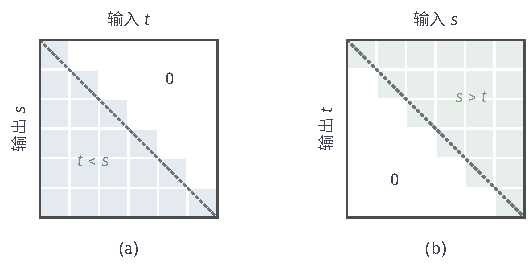
\includegraphics[width=89.623mm]{figures/04-spaces-measures-and-geometry/03-function-spaces/tikz/lop-kernel-adjoint/figure.pdf}
  \caption{积分核与伴随核关于对角线互为镜像，方格表示把区间六等分后的矩阵，虚线是连续极限下的边界，列从左到右、行从上到下对应变量增大。(a)$V$的核$\mathbf 1_{\{t<s\}}$，填色处取值$1$，是下三角矩阵。(b)伴随$V^*$的核$\mathbf 1_{\{s>t\}}$，是上三角矩阵。两核不相等，所以$V$不自伴。}
  \label{fig:lop-kernel-adjoint}
\end{BookInlineFigure}

\subsection{正算子}
\label{sec:lop-positive}

自伴保证二次型$\langle x,Tx\rangle$是实数，但这个实数可正可负。很多场合需要它非负：例如$\langle x,T^*Tx\rangle=\lVert Tx\rVert^2$度量输出的能量。这相当于矩阵的半正定，给出比自伴更强的条件。

\begin{definition}[正算子]
\label{def:lop-positive-operator}
设$T\in\mathcal B(H)$自伴。若
\begin{equation}
 \langle x,Tx\rangle\geq0\qquad(x\in H),
 \label{eq:lop-positive}
\end{equation}
则称$T$为\term{正算子}（positive operator），记作$T\geq0$。
\end{definition}

两个基本例子是正交投影与$T^*T$。对正交投影，
\[
 \langle x,Px\rangle=\langle Px,Px\rangle=\lVert Px\rVert^2\geq0.
\]
对任意$T\in\mathcal B(H_1,H_2)$，$T^*T\in\mathcal B(H_1)$自伴，因为$(T^*T)^*=T^*T^{**}=T^*T$，并且
\[
 \langle x,T^*Tx\rangle=\langle Tx,Tx\rangle=\lVert Tx\rVert^2\geq0.
\]

\paragraph{自伴条件与二次型非负条件}
定义把两个条件分开写出，因为在实空间中二次型非负并不能推出自伴。平面上逆时针旋转$90^\circ$的矩阵
\[
 \bm R=\begin{bmatrix}0&-1\\1&0\end{bmatrix}
\]
满足$\bm x^{\top}\bm R\bm x=-x_1x_2+x_2x_1=0$，二次型非负，却不对称。

复Hilbert空间中情况不同：二次型对一切$x$取实值已经迫使算子自伴。记$B=T-T^*$，它的二次型为
\[
 \langle x,Bx\rangle=\langle x,Tx\rangle-\langle Tx,x\rangle=2\mathrm i\operatorname{Im}\langle x,Tx\rangle=0.
\]

把$x+v$代入$\langle x,Bx\rangle=0$并展开，得到
\[
 \langle x,Bv\rangle+\langle v,Bx\rangle=0.
\]
再把$v$换成$\mathrm iv$，由第一个变量的共轭线性，得到
\[
 \mathrm i\langle x,Bv\rangle-\mathrm i\langle v,Bx\rangle=0.
\]
两式合起来给出$\langle x,Bv\rangle=0$对一切$x,v$成立，所以$B=0$。

为了使定义在实、复两种情形下一致，我们仍把自伴列为前提。反过来，自伴也不推出二次型非负，下面的积分算子就是例子。

\paragraph{积分算子的正性}
对$L^2(\mu)$上满足$k(x,y)=\overline{k(y,x)}$的平方可积核，自伴积分算子的正性由积分二次型检验：
\begin{equation}
 \langle f,Tf\rangle=\iint\overline{f(x)}\,k(x,y)\,f(y)\,\mathrm d\mu(y)\,\mathrm d\mu(x)\geq0\qquad(f\in L^2(\mu)).
 \label{eq:lop-integral-positive}
\end{equation}
这是矩阵半正定条件$\bm f^*\bm K\bm f\geq0$的连续版本。

贯穿例子中，
\[
 \langle f,Tf\rangle=\Bigl\lvert\int f\,\mathrm d\mu\Bigr\rvert^2+\Bigl\lvert\int zf\,\mathrm d\mu\Bigr\rvert^2\geq0,
\]
所以它是正算子。把核换成$1-6xz$，算子仍自伴，但取$f=x$，由$\int z\,\mathrm d\mu=0$与$\int z^2\,\mathrm d\mu=1/3$得
\[
 Tf=-2x,\qquad\langle f,Tf\rangle=-2\int x^2\,\mathrm d\mu=-\frac23<0,
\]
它不是正算子。

\paragraph{核逐点非负不等于正算子}
矩阵元素全为正的矩阵未必半正定，核也是如此。取两点集合$\{1,2\}$配计数测度，此时$L^2$就是$\mathbb F^2$，积分就是求和。核$k(1,1)=k(2,2)=0$、$k(1,2)=k(2,1)=1$逐点非负且对称，对应的算子交换两个坐标，矩阵为$\left[\begin{smallmatrix}0&1\\1&0\end{smallmatrix}\right]$。

取$f=(1,-1)$，$Tf=(-1,1)$，于是$\langle f,Tf\rangle=-2<0$。

反方向也不成立：核$k(x,z)=xz$在$x=1,z=-1$处为负，却给出
\[
 \langle f,Tf\rangle=\Bigl\lvert\int zf\,\mathrm d\mu\Bigr\rvert^2\geq0
\]
的正算子。正性是关于所有输入的二次型的条件，不能由核在单个点上的符号判断。
